\documentclass{article}
\usepackage{apamposter_1}
\usepackage[square,numbers]{natbib}
\usepackage{lmodern}
\usepackage{textpos}
\setcounter{secnumdepth}{2}
\newcommand{\nb}[1] {\textcolor{red}{#1}}
\setlength{\TPHorizModule}{1in}
\setlength{\TPVertModule}{1in}
\begin{document}
\bibliographystyle{plainnat}
%\begin{center}
%
% Start of title...
%
% switch into sans-serif for title

\begin{textblock}{62}(0,0)

%\textblockcolor{white}

\begin{center}

\vspace{5mm}\def\myfig#1{\begin{center}\includegraphics[width=\graphicswidth]{#1}\end{center}}

{\VeryHuge\color{black} \textbf{Design, Fabrication, Installation and First Results of the HBT-EP Shaping Coil}}

\vspace{15mm}
\rm
\sf
\LARGE\textbf{\color{lnavy}
P. Byrne$^\dagger$, J. P. Levesque, D. Rhodes, Q. Peng, G. Navratil, M. E. Mauel \hspace{2in} \emph{Columbia University}}\\

\vspace{5mm}

\end{center}
\end{textblock}
\begin{textblock}{12}(49,3)
\begin{flushright}

{\color{black}$^{\dagger}$email: {pjb2132@columbia.edu} }\hspace{.25in}

\end{flushright}
\end{textblock}

\begin{textblock}{3}(.2,.75)


\includegraphics[scale =.75]{CU_logo_exported.png}

\end{textblock}


\begin{textblock}{1}(57,.45)


\includegraphics[scale =1]{hbt_logo.png}

\end{textblock}


\vspace{100mm}
\hrule{}
\vspace{10mm}

% End of title, start of content..

%\fbox{\parbox[b][4em][t]{0.33\textwidth}{Some \\ text} }
%\fbox{\parbox[c][4em][s]{0.33\textwidth}{Some \vfill text} }
%\fbox{\parbox[t][4em][c]{0.33\textwidth}{Some \\ text} }

%\begin{minipage}[b][5\baselineskip][b]{3in}
  %%\centering
  %%\vspace{.25in}
  %%\begin{flushleft}
  %
\includegraphics[width=3in]{CU_logo_exported.png}
  %%\end{flushleft}
%\end{minipage}
%\begin{minipage}[t][5\baselineskip][t]{.75\textwidth}
    %\centering
    %\VeryHuge{\textbf{
%Design, Fabrication, Installation and First Results of the HBT-EP Shaping Coil}}\\
    %\vspace{.25in}
    %\Huge{\textbf{\color{lnavy}
%P. Byrne, J. P. Levesque, D. Rhodes, Q. Peng, G. Navratil, M. E. Mauel \hspace{2in} Columbia University}}
%\end{minipage}
%\begin{minipage}[b][5\baselineskip][b]{3in}
  %\begin{flushright}
  %\vspace{.25in}
  %
\includegraphics[width=3in]{hbt_logo.png}
  %\end{flushright}
%\end{minipage}
%%\includegraphics{leftlogo}\hfill Text\hfill\includegraphics{rightlogo}
%%\VeryHuge{\textbf{
%%Design, Fabrication, Installation and First Results \\
%%of the HBT-EP Shaping Coil}}\\
%%\vspace{.25in}
%%\Huge{\textbf{
%%P. Byrne, J. P. Levesque, D. Rhodes, Q. Peng, G. Navratil, M. E. Mauel \hspace{3in} Columbia University}}
%%\end{center}
%%\begin{flushright}
%%
\includegraphics[width=0.075\columnwidth]{hbt_logo.png}
%%\end{flushright}
%\vspace{.25in}
%%\end{VeryHuge}
\begin{multicols}{5}
\section{Abstract}
%\begin{itemize}
A low self-and-mutual inductance, zero net turn coil and its capacitive power supply have been fabricated and installed on the HBT-EP Tokamak.  The coil will locally shape HBT-EP's normal circular cross section, up to and including the creation of a poloidal field null above the inboard midplane.  This will enable HBT-EPs first investigation of the effects of shaping on the MHD multimode spectrum.  Post installation tests have affirmatively proven the ability of the coil to impose a continuum of shaping, from circular to fully diverted. A description of the coil system, it's components, and qualifying tests are below.  Results of initial experiments with are also provided and compared with simulations.\\
\section{Motivation}
\begin{itemize}
\item Simulations of shaped and unshaped plasmas using TokaMac and DCON show change in expected resonant plasma modes
\item MHD multimode response shows decoupling of multimode effects with shaping.\\
\begin{center}
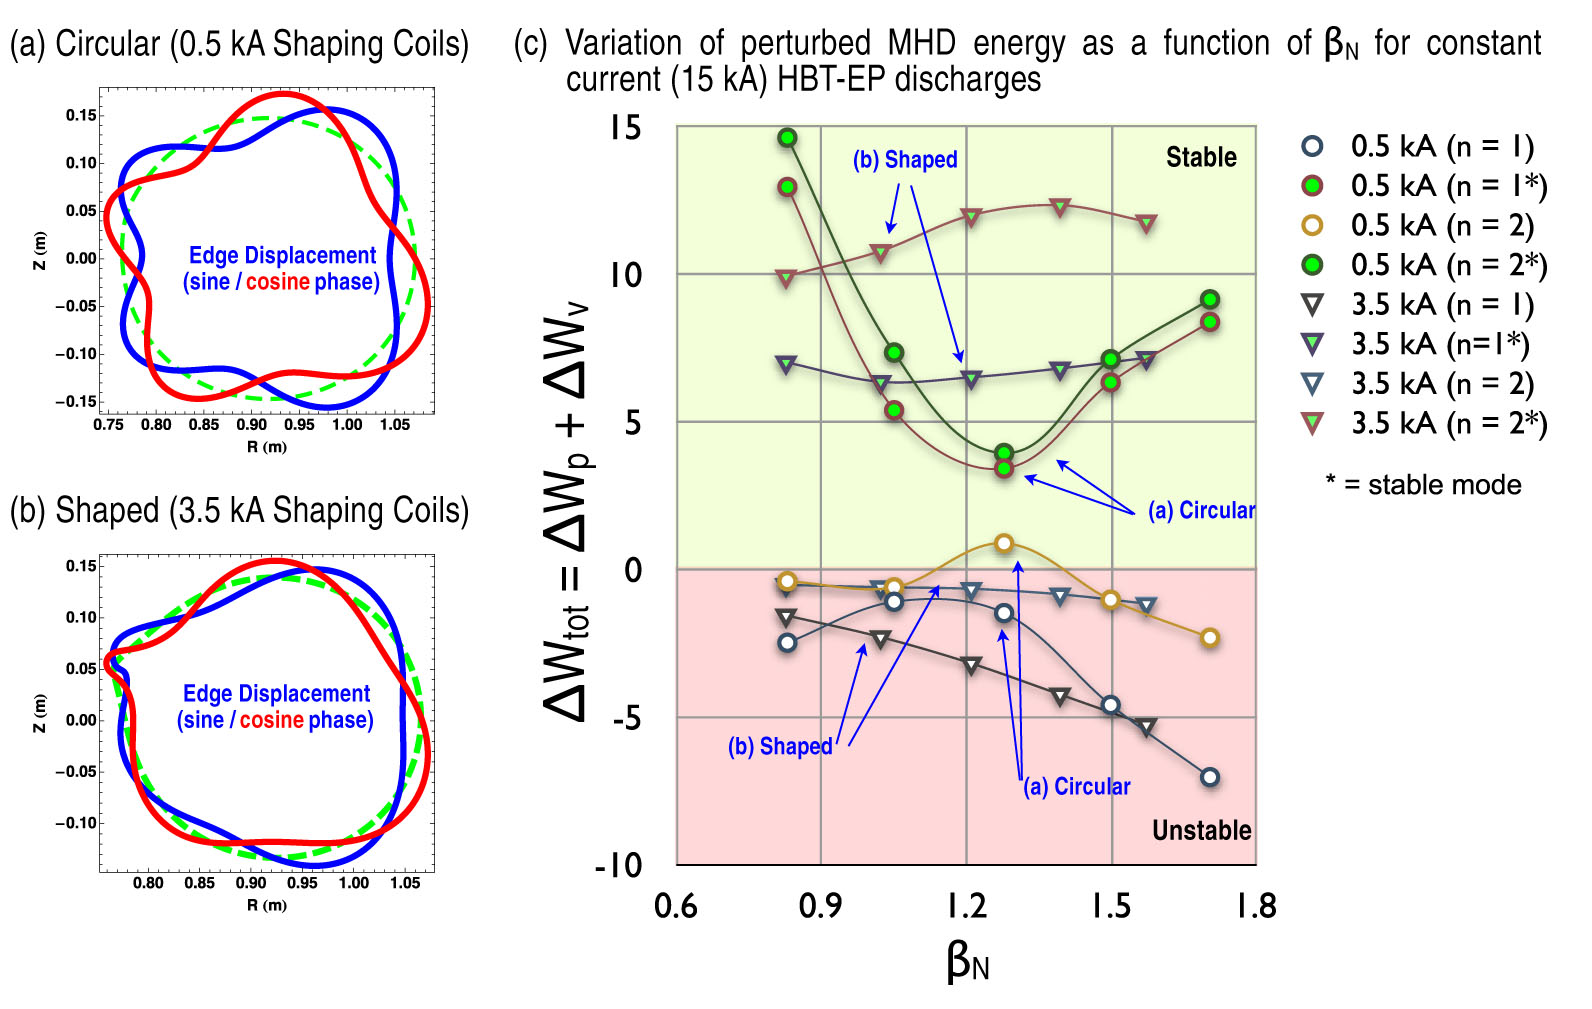
\includegraphics[width=0.9\columnwidth]{ModeDWimage2}\\
\vspace{.25in}
Fig. 1\\
Unstable and ``most marginal" modes modeled in DCON for n = 1 and n = 2 in circular and shaped plasmas.\\
\end{center}
\item There is a strong multimode response across all modes for the unshaped plasma when  $\beta$$_n$ rises past 1.2 (correlates to q$_a$=3).  Beta was scanned by taking a typical HBT-EP plasma equilibria and varying the core pressure$^{[1]}$

%\begin{center}Calculation of MHD multimode response for shaped and unshaped plasma.\\
%4 modes are observed for circular and shaped plasmas, the unstable mode \\
%and the "most marginal" modes for the cases n = 1 and n = 2. There is a \\
%strong multimode response across all modes for the unshaped plasma when \\
%$\beta$$_n$ rises past 1.2 (correlates to q$_a$=3).  Beta was scanned by taking a typical \\
%HBT-EP plasma equilibria and varying the core pressure\end{center}

\end{itemize}
\section{Design and Fabrication}
\subsection{The Coil}
\begin{itemize}
\item The HBT-EP shaping coil provides up to 40kA-turns of current.  HBT-EP's usual I$_{\mbox{plasma}}$ is ~10-15kA
\item The coil consists of a single 1$/$0 welding wire, wound toroidally 8 times. It is located slightly above the high field side midplane.
\item The 8 loops are distributed into 3 bundles, consisting of 2, 4, and 2 windings.
\item The winding reverses direction twice, such that the central 4-loop bundle carries current in thhe opposite direction from the flanking 2-loop bundles.
\item Zero-Net-Turns design reduces coil self (L) and mutual (M) inductance
\item Low L allows fast turn on, and high-current operation with low energies
\item Low M reduces the shaping coil's interference with existing magnetics, and localizes the plasma shaping to a few poloidal degrees from coil center.\\
\begin{center}
%\vspace{.25in}
\columnbreak
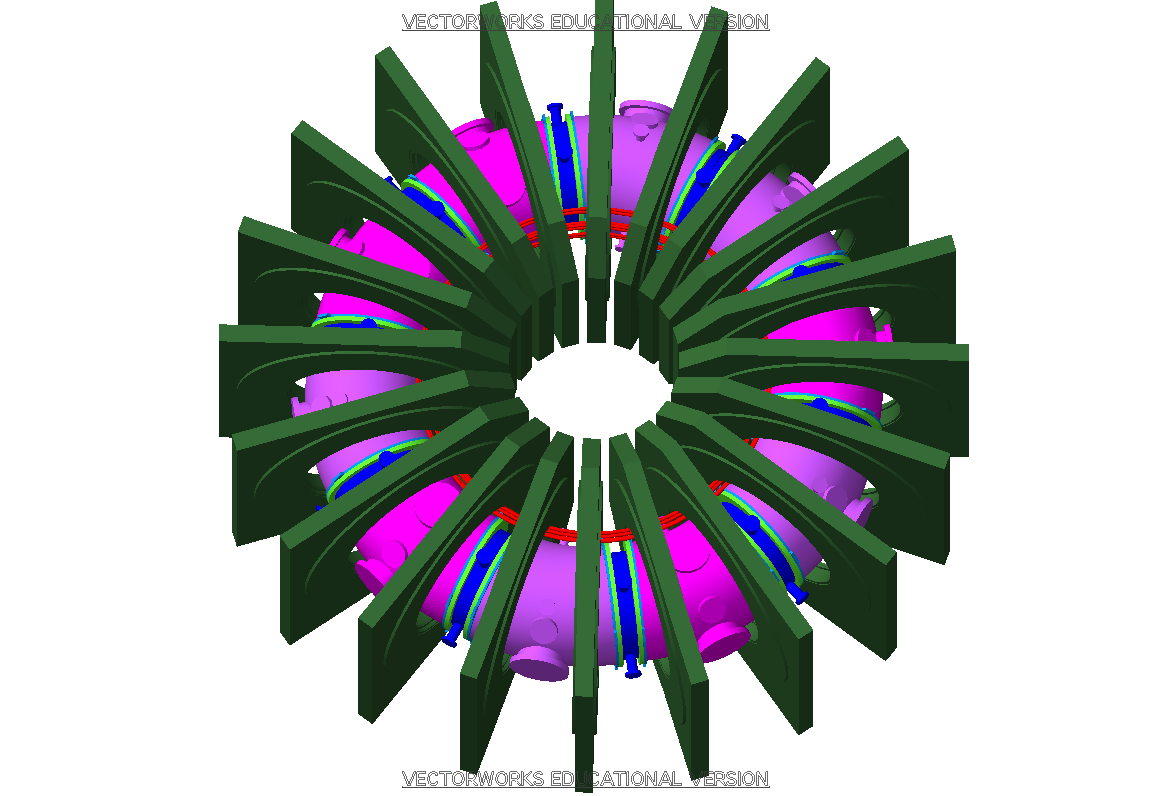
\includegraphics[width=0.9\columnwidth]{HBT-EP_Full2.pdf}
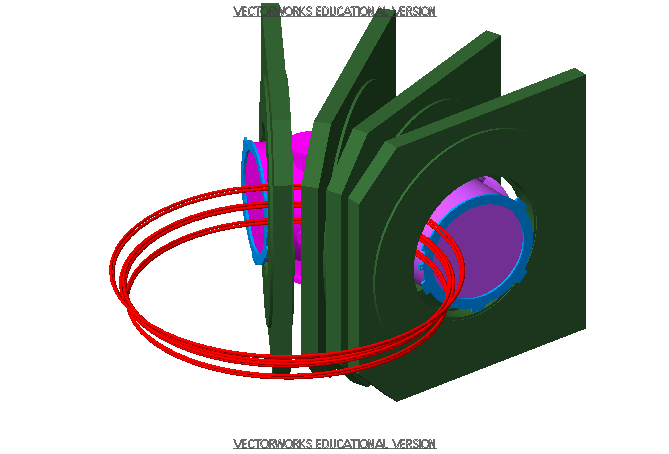
\includegraphics[width=0.9\columnwidth]{HBT-EP_Section.pdf}\\
Fig. 2\\
Full and sectioned views of the HBT-EP Tokamak\\
with the new shaping coil installed\\
%\vspace{.25in}
\end{center}
\item The coil's low inductance (42$\mu$H) and low resistance($<$50m$\Omega$) allow for the use of a low energy, low voltage power supply.
%\columnbreak
\subsection{The Power Supply}
\item The shaping fields are sustained by capacitive discharge, provided by a 900V, 7.5mF startup bank, and a 250V, 0.6F crowbar bank.  
\item The capacitors are fired in two-stages, the start bank providing a quick establishment (850$\mu$s) and the crowbar bank long sustainment (90$\%$ of max current after 6ms) of the shaping field.\\
\vspace{.25in}
\begin{center}
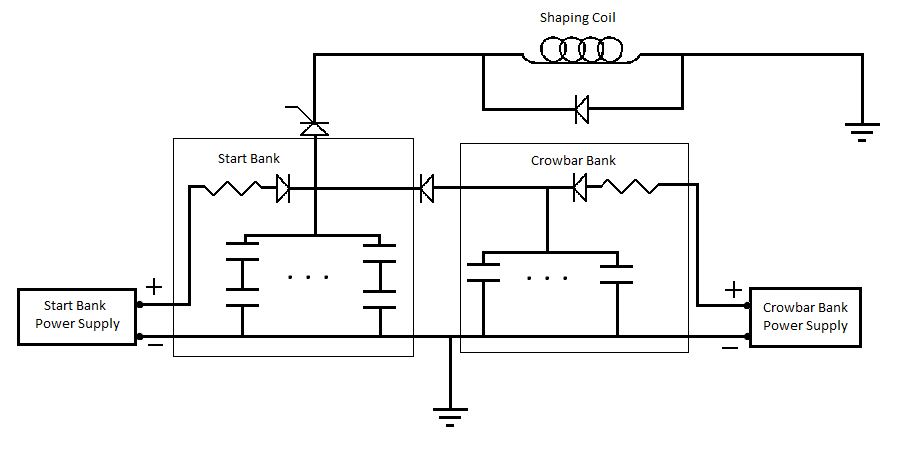
\includegraphics[width=0.8\columnwidth]{Simplified_bank_diagram.png}
\newline
Fig. 3\\
Diagram of the HBT-EP shaping circuit.\\
Start bank is high voltage, fast risetime.\\
Crowbar bank is low voltage, high capacitance.\\
%\vspace{.25in}
\end{center}
\columnbreak
\item The power supply provides up to 40kA-turns of shaping current with only 22kJ of energy thanks to impedance minimizing design.
\item The crowbar bank is passively soft-switched into the circuit using a high current rectifier, making a smooth transition from start-up to steady-state regimes\\
\vspace{.25in}
%\columnbreak
\begin{center}
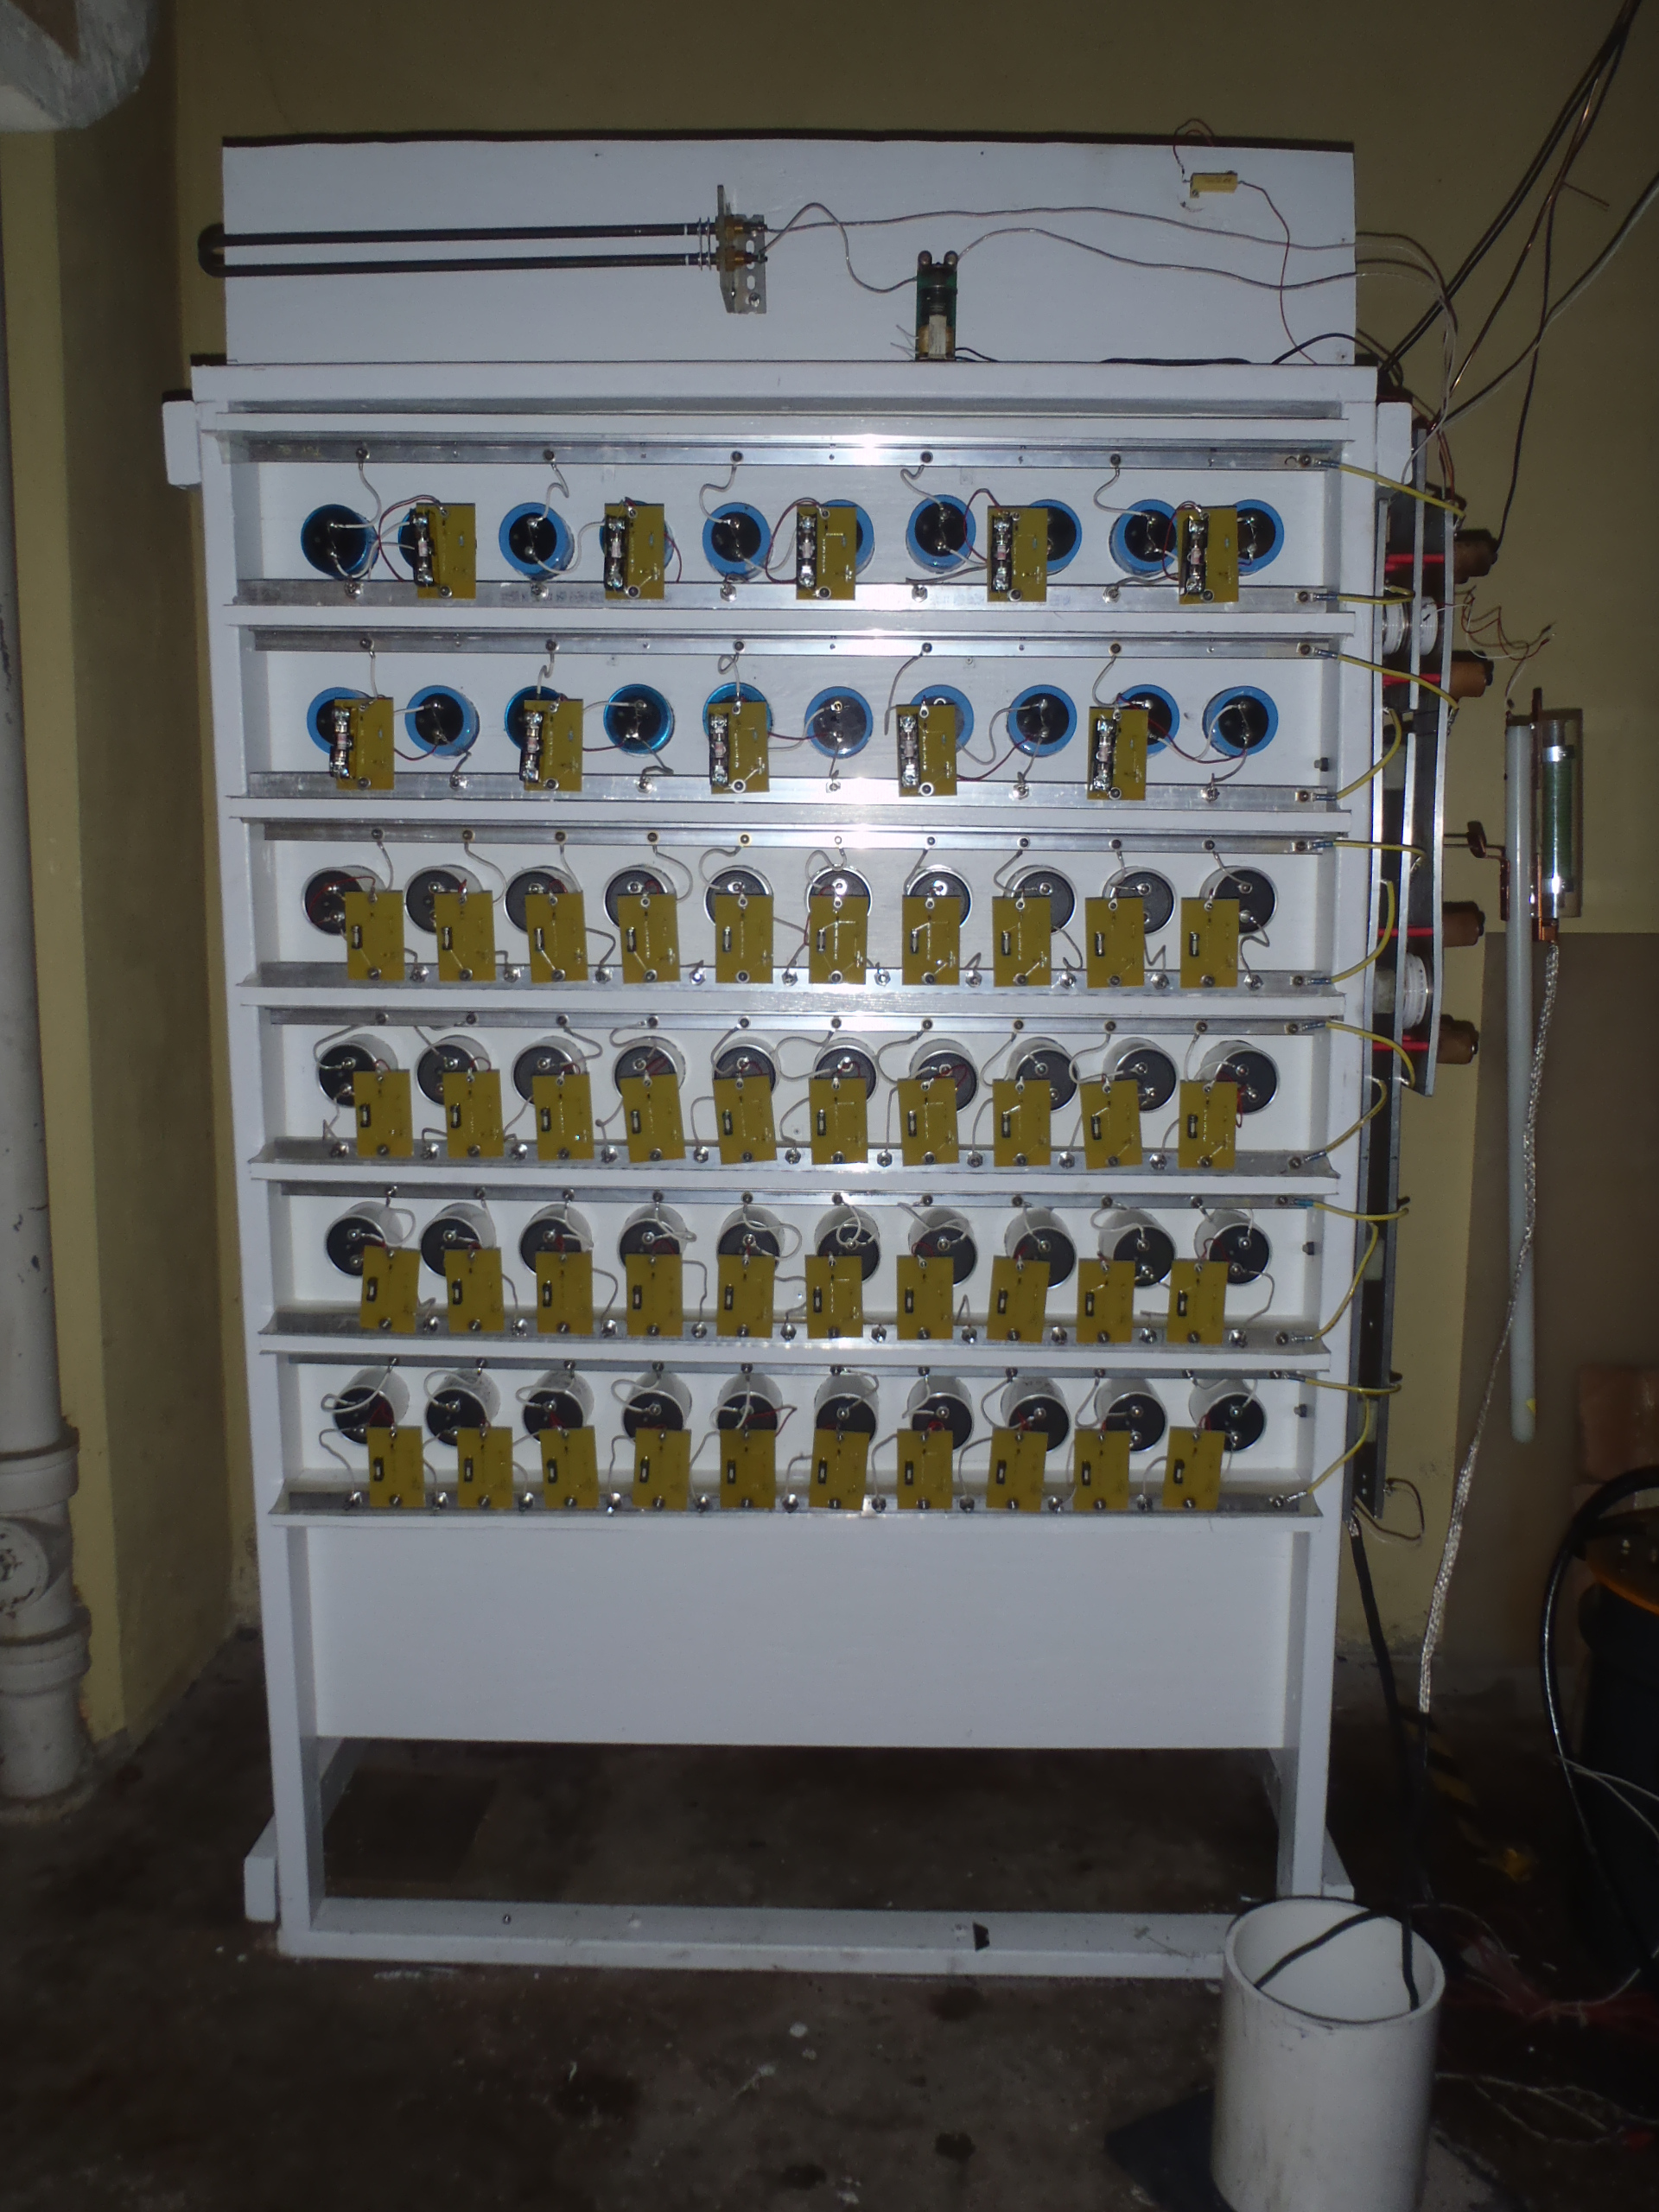
\includegraphics[width=0.8\columnwidth]{Cap_bank.jpg}\\
Fig. 4\\
The HBT-EP shaping power supply\\
Start bank caps are blue, crowbar bank caps are white\\
Low required operating energy allows for compact construction\\
\vspace{.25in}
\end{center}
%\columnbreak
\subsection{The Limiter}
\item HBT-EP has two poloidally complete Mirnov coil arrays (see Fig.'s 6 and 7 for location)
\item Diverted plasmas will release significant energy to the area near the x-point.
\item HBT-EP's existing limiters were designed for a circular plasma, they limit at the midplane and top/bottom of the plasma
\item Two divertors were installed near the poloidal arrays to shade the sensors from incoming plasma\\
\begin{center}
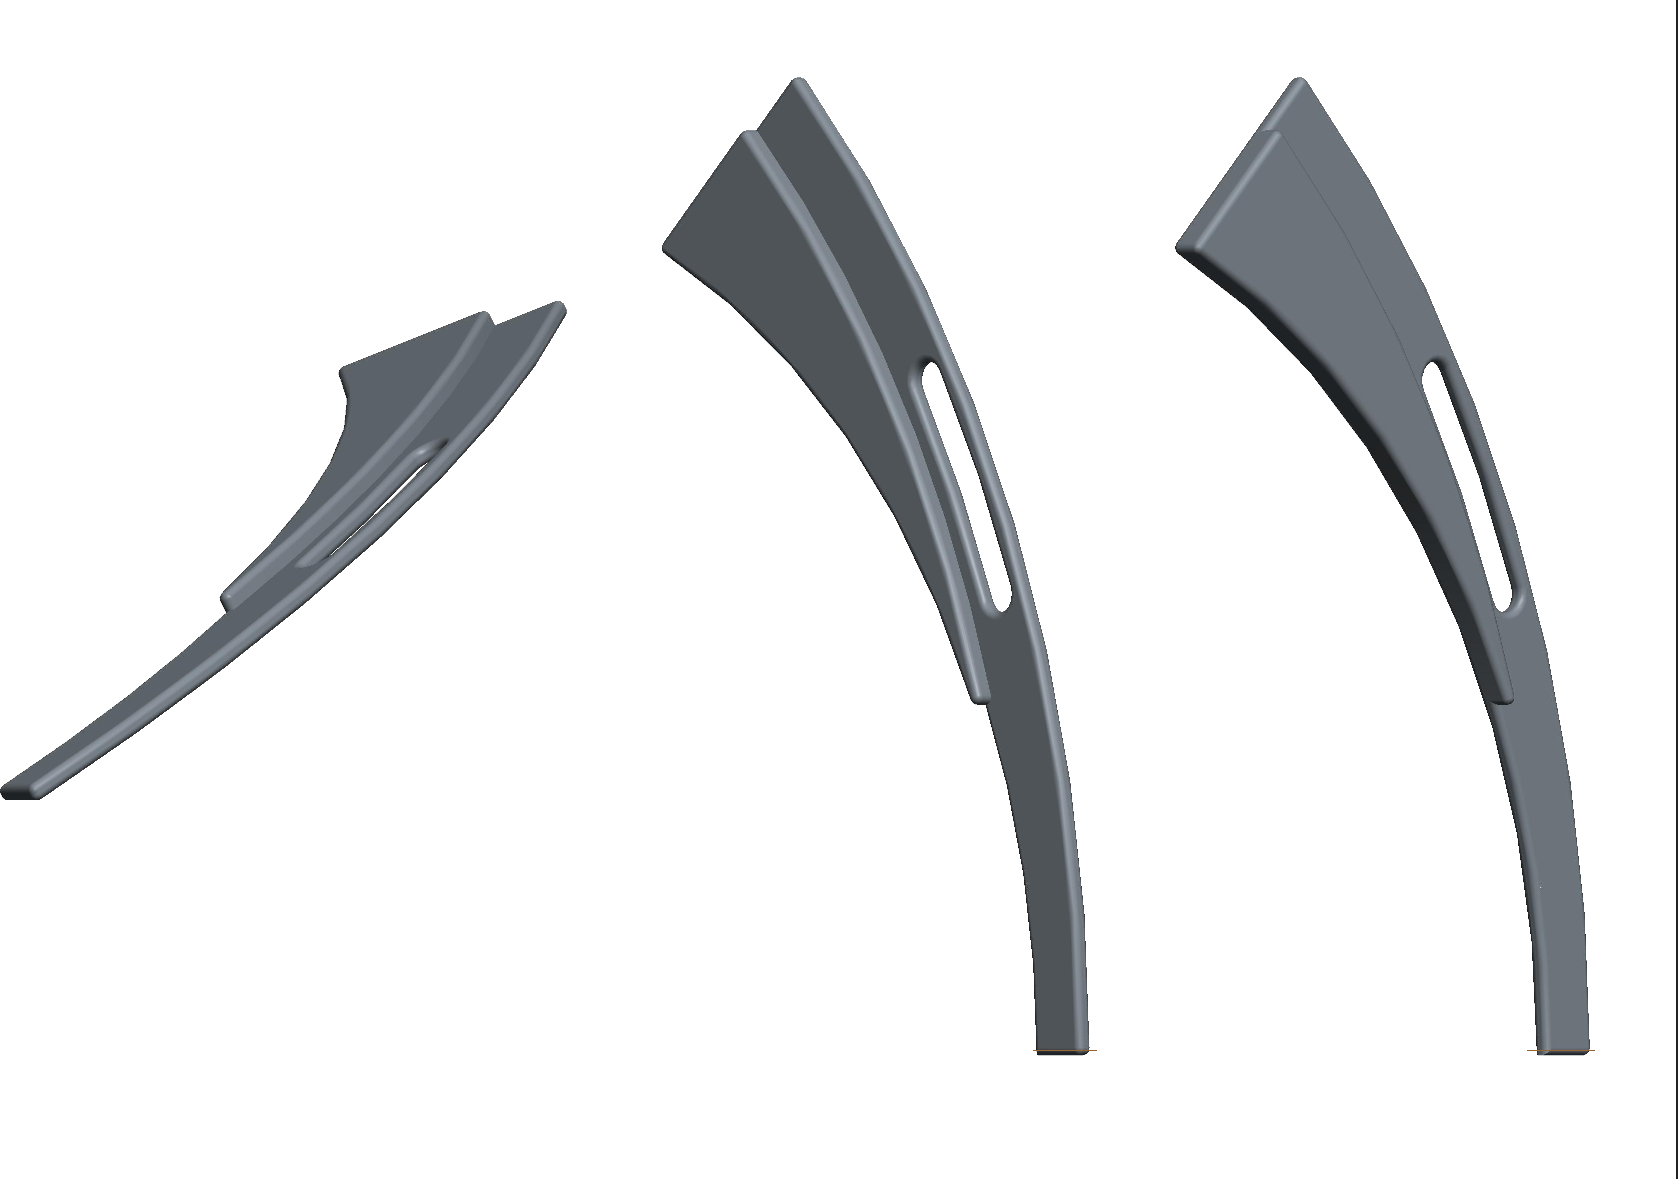
\includegraphics[width=0.5\columnwidth]{strike_point_limiter_cropped.pdf}\\
Fig. 5\\
The limiters are $1/4^{``}$ 3-16 Stainless Steel\\
They shield 45$^\circ$ of poloidal angle, rising from the inboard midplane.
\end{center}
\end{itemize}
\columnbreak
\section{Operation and Qualification}
\subsection{SPICE Simulations}
\begin{itemize}
\item Pulse amplitude and shape are controlled by the voltages on each bank; allows control of startup speed, tracking of shaping current to plasma current and/or position, and degree of plasma shaping - up to and including a fully diverted discharge.
\item Voltages and capacitances selected in design phase via SPICE to allow a maximum shaping current of ~9kA/turn\\
%\vspace{.25in}
\begin{center}
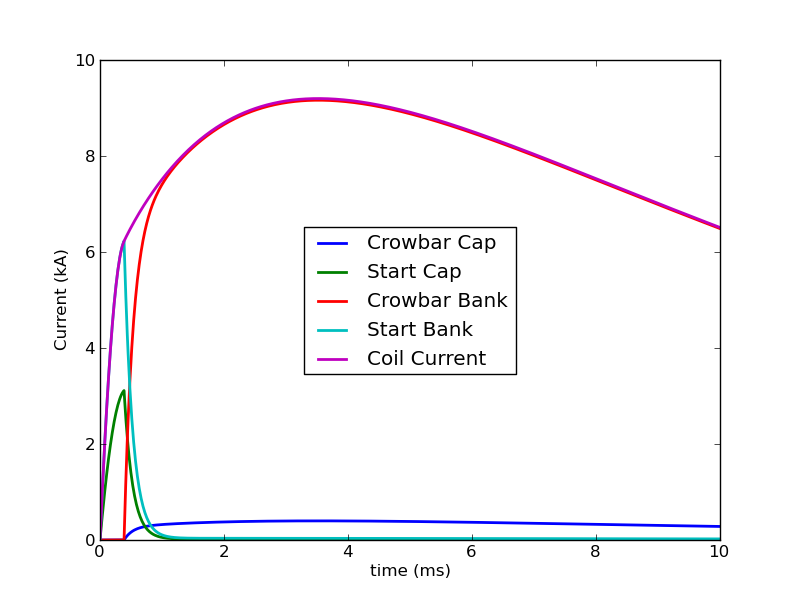
\includegraphics[width=0.75\columnwidth]{bank_currents.png}\\
Fig. 6\\
SPICE simulation of cap bank discharge at maximum voltage\\
Passive switching allows smooth transition to crowbarred operation\\
\end{center}
\vspace{.25in}
%\columnbreak
\subsection{Post Construction}
\item Shaping current is monitored by means of a rogowski coil manufactured in-house.
\item Comparison of simulated pulse traces to actual operation shows higher current than expected.
\item Design points of coil were 49$\mu$H, 22m$\Omega$. Inductance measured @ 42 $\mu$H, resistance of but 17-18m$\Omega$ can be inferred from pulse shape.
\item Transition from startup to crowbar operation is bumpier than predicted, but still much smoother than possible with active switching\\
\begin{center}
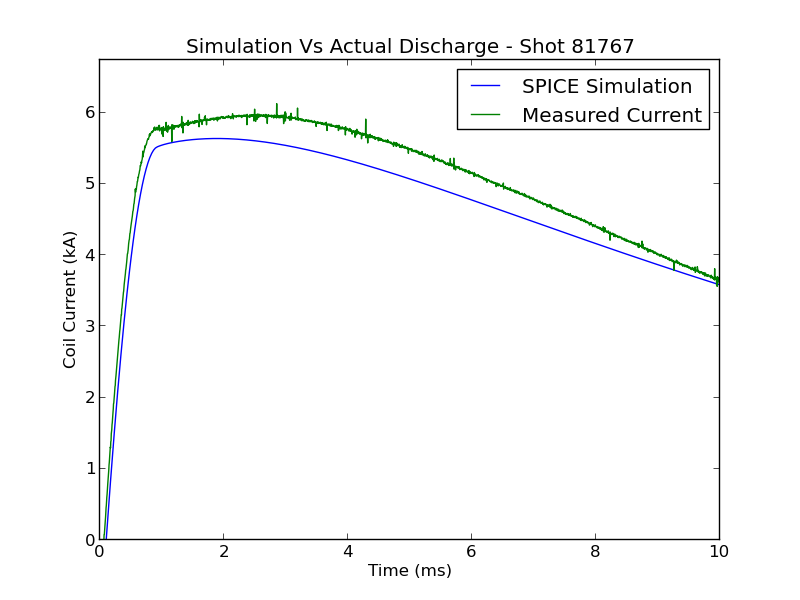
\includegraphics[width=0.75\columnwidth]{shaping_current_sim_vs_real_81797.png}\\
Fig. 7\\
SPICE simulation of standard discharge\\
compared to current as meaured in the coil\\
\end{center}
%\columnbreak
%\columnbreak
\subsubsection{Modeling of flux surfaces suggests HBT-EP has been successfully run diverted, at 70$\%$ power}
%\vspace{.25in}
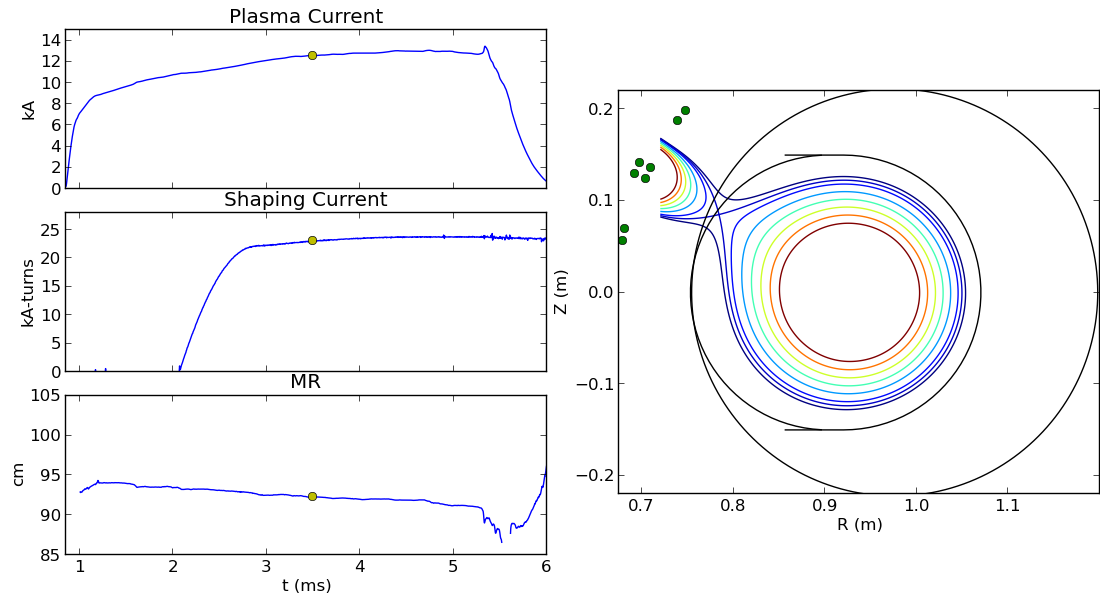
\includegraphics[width=0.85\columnwidth]{flux_surfaces_during_shaping.png}
\begin{center}
Fig. 8\\
Filament-current flux surface reconstruction using data from HBT-EP shot 81597\\
Black lines represent vacuum chamber and poloidal sensor array/plasma limiting surface\\
Green dots represent physical location of shping coil turns\\
\end{center}
%\vspace{.25in}
%\columnbreak
\item Toroidal non-axisymmetries are presentunavoidable due to high density of pre-existing diagnostics in the coil path.\\
\newline
%\vspace{.25in}
\begin{center}
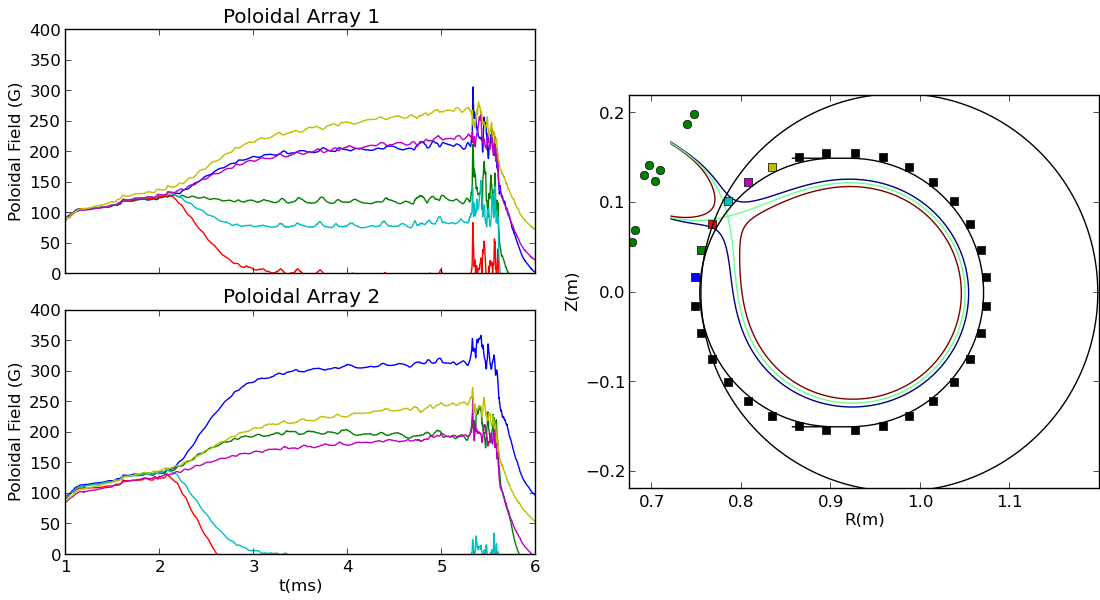
\includegraphics[width=0.85\columnwidth]{poloidal_field_cancellation_APS_2013.png}\\
Fig. 9\\
Poloidal field measured at two toroidal locations near HBT-EP x-point for shot 81597.\\
$B_p$ traces are color coded to the sensors as shown on the right.\\
\end{center}
%\item The plasma is still diverted, but will have a larger scrape-off layer than otherwise
%\item Plasmas being shaped are more susceptible to diversion, but shots have been taken with steady MR, that are not extreme outboard.
%\item Study of decay index last year showed that we should be able to develop a stable shot.
%\item Mode analysis is so far inconclusive, as the spectra of diverted shots do not seem significantly different from limited ones
%\item future work: develop a longer lived diverted discharge
%\item future work: increase the database of diverted plasmas
%\item future work: search the database for or develop an unshaped shot with similar parameters (MR,IP,q*) for a direct comparison to diverted discharges
%\item future work: work to understand, and if possible, mitigate the toroidal asymmetries in the coil
%\item plots to display:
%\item MR (and IP ?) trace for a 'hard crash' shaped shot
%\item comparison of simulation of bfields tree data at TA
%\item stripey plot of shaped q=3 shot: best of 81593-98 compared to stripey plot of unshaped q=3 shot
%\item BD dominant modes and spatial structures from shaped to unshaped

%\begin{center}Calculation of MHD multimode response for shaped and unshaped plasma.\\
%4 modes are observed for circular and shaped plasmas, the unstable mode \\
%and the "most marginal" modes for the cases n = 1 and n = 2. There is a \\
%strong multimode response across all modes for the unshaped plasma when \\
%$\beta$$_n$ rises past 1.2 (correlates to q$_a$=3).  Beta was scanned by taking a typical \\
%HBT-EP plasma equilibria and varying the core pressure\end{center}
%\columnbreak
\end{itemize}
\section{Future Work}
\begin{itemize}
\item Investigate the multimode spectum of shaped HBT-EP plasmas, specifically the effects of degree of shaping on MHD modes.
\item Characterize and understand the cause of these differences, and extrapolate to the performance of advanced Tokamaks such as ITER or DEMO
\end{itemize}
\section{Summary}
\label{sec:summary}
\begin{itemize}
\item A shaping coil has been installed on HBT-EP, opening the door to diverted operation
\item Low-Z design ensures the standard HBT-EP discharge in non-shaped plasmas is unaltered
\item Test runs have demonstrated diverted operation to be within reach.
\end{itemize}

\section{Acknowledgements}
Design, fabrication and installation were all aided greatly by the contributions of Nick Rivera and James Andrello.\\
This work was supported by DOE grant DE-FGO2-86ER53222.
\bibliography{literature.bib}
\end{multicols}
\end{document}

